\documentclass{beamer}
\beamertemplatenavigationsymbolsempty
\usefonttheme[stillsansseriflarge]{serif}
\setbeamertemplate{footline}[frame number]
\usepackage[type1]{libertine}
\usepackage{bbold}
\usepackage{tikz}
\usepackage{feynmp-auto}
\usepackage{subfig}
\usepackage{pgfplots}

\author{Shih-Kai Lin}
\institute[UM]{Colorado State University}

\title{\texorpdfstring{$\bar{\nu}_\mu$}{numubar} Charged Current Inclusive Cross Section Measurement with NO$\nu$A Near Detector}
\date{June 7, 2016}
\begin{document}
  \unitlength = 1mm
\begin{frame}
\titlepage
\end{frame}

\begin{frame}{Why Cross Section Measurement}
\begin{itemize}
\item essential in all neutrino experiments
\item needed in the interpretation of neutrino oscillation data
\item Historical measurements in the oscillation-relevant energy range, $E_\nu<30$ GeV, have uncertainties of the order of $10\%$.
\item Modern neutrino experiments make use of nuclear targets to increase event yields, which are less understood with nuclear effects.
\end{itemize}
\end{frame}

\begin{frame}{Neutrino Interactions}
\begin{figure}[ht!]
  \centering
  \subfloat{
		\begin{fmffile}{nuCC}
		  \begin{fmfgraph*}(40,25)
		    \fmfpen{thick}
				\fmfleft{i1,i2}
				\fmfright{o1,o2}
				\fmfbottom{b}
				\fmf{fermion,label=$\nu_\ell/\bar{\nu}_\ell$}{i2,v1}
				\fmf{fermion,label=$\ell^{-/+}$}{v1,o2}
				\fmf{boson,label=$W^{+/-}$}{v1,b}
			\end{fmfgraph*}
		\end{fmffile}
  }
  \subfloat{
		\begin{fmffile}{qCC}
		  \begin{fmfgraph*}(40,25)
		    \fmfpen{thick}
				\fmfleft{i1,i2}
				\fmfright{o1,o2}
				\fmfbottom{b}
				\fmf{fermion,label=$\nu_\ell/\bar{\nu}_\ell$}{i2,v1}
				\fmf{fermion,label=$\nu_\ell/\bar{\nu}_\ell$}{v1,o2}
				\fmf{boson,label=$Z^0$}{v1,b}
			\end{fmfgraph*}
		\end{fmffile}
  }
\end{figure}
\begin{figure}[ht!]
  \captionsetup[subfloat]{labelformat=empty}
  \centering
  \subfloat[][charged current\\ flavor changing]{
		\begin{fmffile}{nuNC}
		  \begin{fmfgraph*}(40,25)
		    \fmfpen{thick}
				\fmfleft{i1,i2}
				\fmfright{o1,o2}
				\fmftop{t}
				\fmf{fermion,label=$q$}{i1,v1}
				\fmf{fermion,label=$q'$}{v1,o1}
				\fmf{boson,label=$W^{+/-}$}{v1,t}
			\end{fmfgraph*}
		\end{fmffile}
  }
  \subfloat[][neutral current\\ flavor conserving]{
		\begin{fmffile}{qNC}
		  \begin{fmfgraph*}(40,25)
		    \fmfpen{thick}
				\fmfleft{i1,i2}
				\fmfright{o1,o2}
				\fmftop{t}
				\fmf{fermion,label=$q$}{i1,v1}
				\fmf{fermion,label=$q$}{v1,o1}
				\fmf{boson,label=$Z^0$}{v1,t}
			\end{fmfgraph*}
		\end{fmffile}
  }
\end{figure}
\end{frame}

\begin{frame}{Neutrino-Nucleon Charged Current Interactions}
\begin{itemize}
  \item quasi-elastic scattering: (target changes but no break up)
  \begin{equation*}
  \nu_\mu+n\rightarrow \mu^- +p
  \end{equation*}
  \item nuclear resonance production: (target goes to excited state, $N^*$ or $\Delta$)
  \begin{eqnarray*}
  \nu_\mu+n\rightarrow \mu^- +p+\pi^0\\
  \nu_\mu+n\rightarrow \mu^- +n+\pi^+
  \end{eqnarray*}
  \item deep-inelastic scattering: (nucleon broken up)
  \begin{equation*}
  \nu_\mu+quark\rightarrow \mu^- +quark'
  \end{equation*}
  \item ``Inclusive" means all channels combined. Any event with an outgoing muon is included.
\end{itemize}
\end{frame}

\begin{frame}{How to Measure Total Cross Section}
\begin{equation*}
\sigma(E)=\frac{\left(N_s(E)-N_b(E)\right)/\epsilon(E)}{\phi(E)N_t}
\end{equation*},
where\\
$\sigma(E)$ is the total cross section ($cm^2$),\\
$N_s(E)$ is the selected number of events,\\
$N_b(E)$ is the background number of events,\\
$\epsilon(E)$ is the selection efficiency,\\
$\phi(E)$ is the neutrino flux, and\\
$N_t$ is the areal number density of the target nucleus ($cm^{-2}$)
\end{frame}

\begin{frame}{Measurements to Date}
\begin{figure}
  \centering
  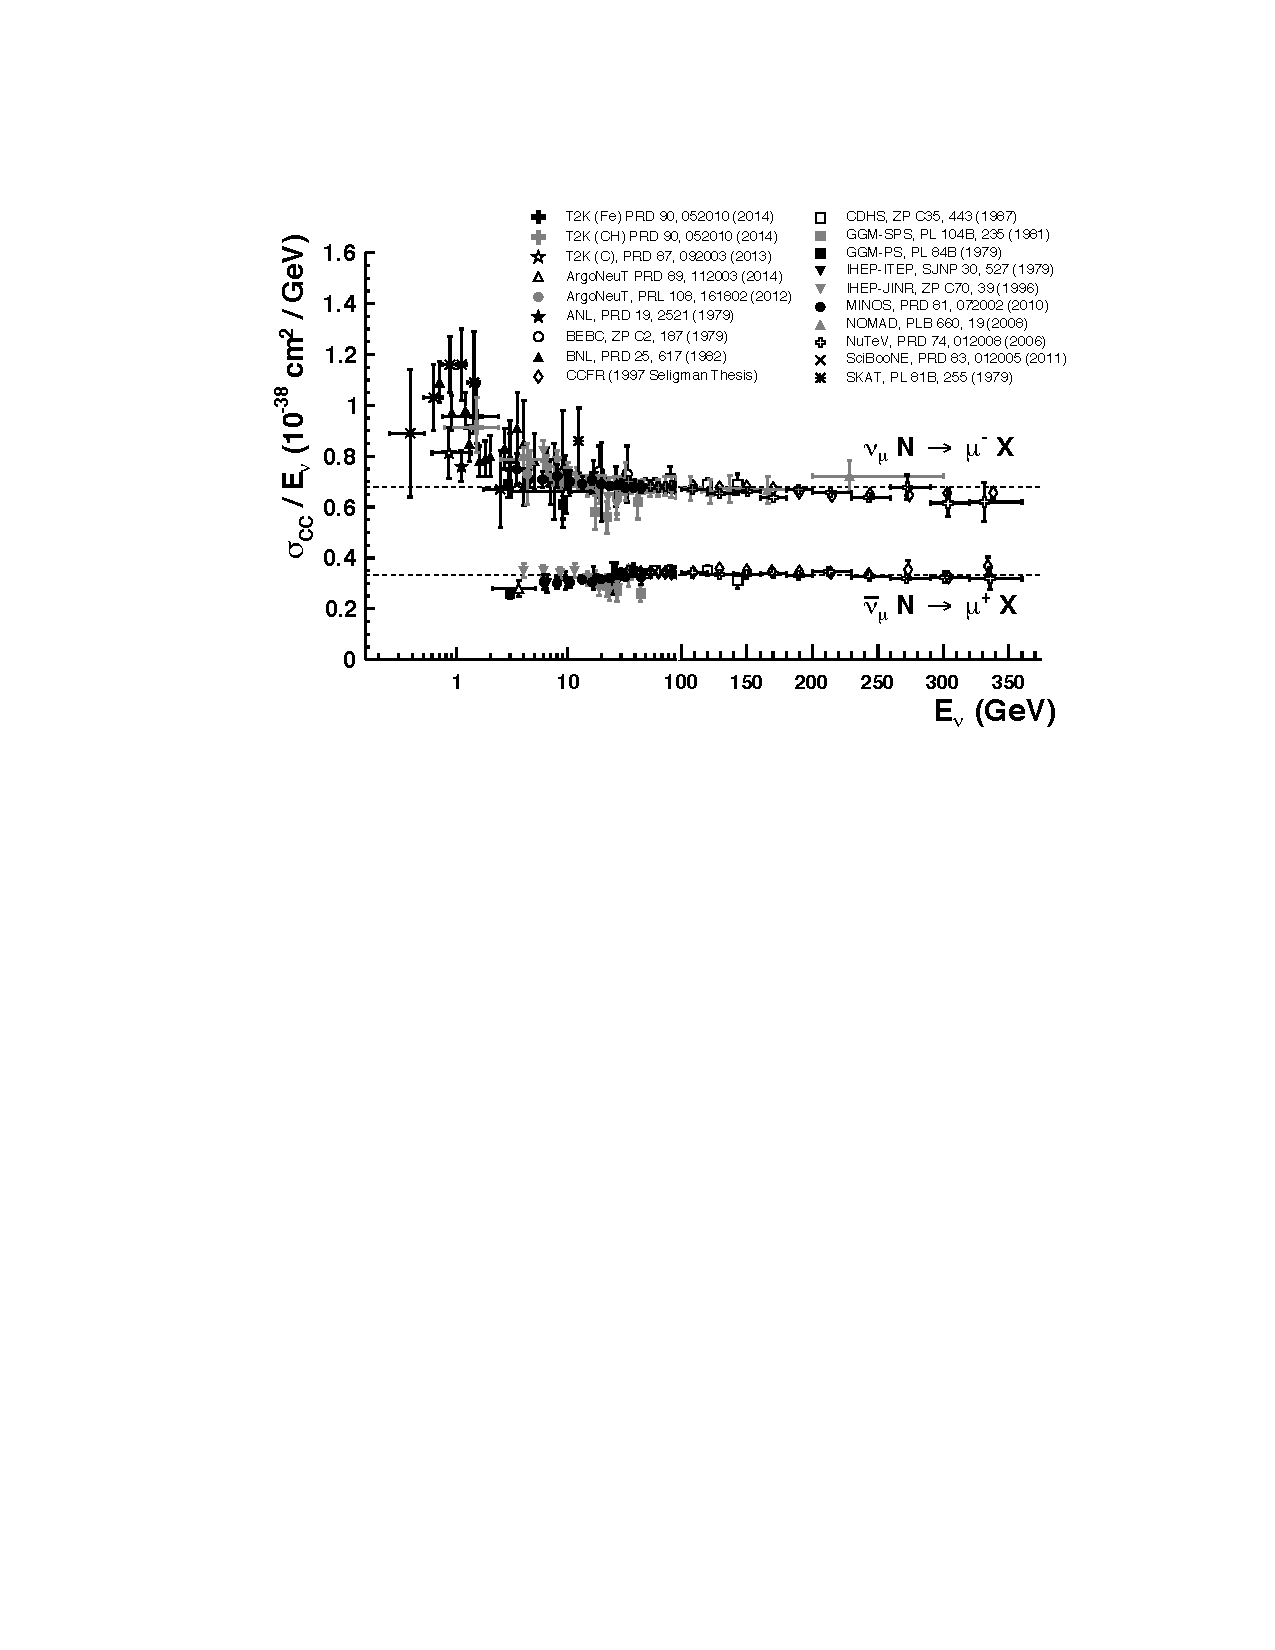
\includegraphics[width=\textwidth]{figures/xsec.pdf}
\end{figure}
\end{frame}

\begin{frame}{Where Do the Neutrinos Come From}
\begin{figure}
\centering
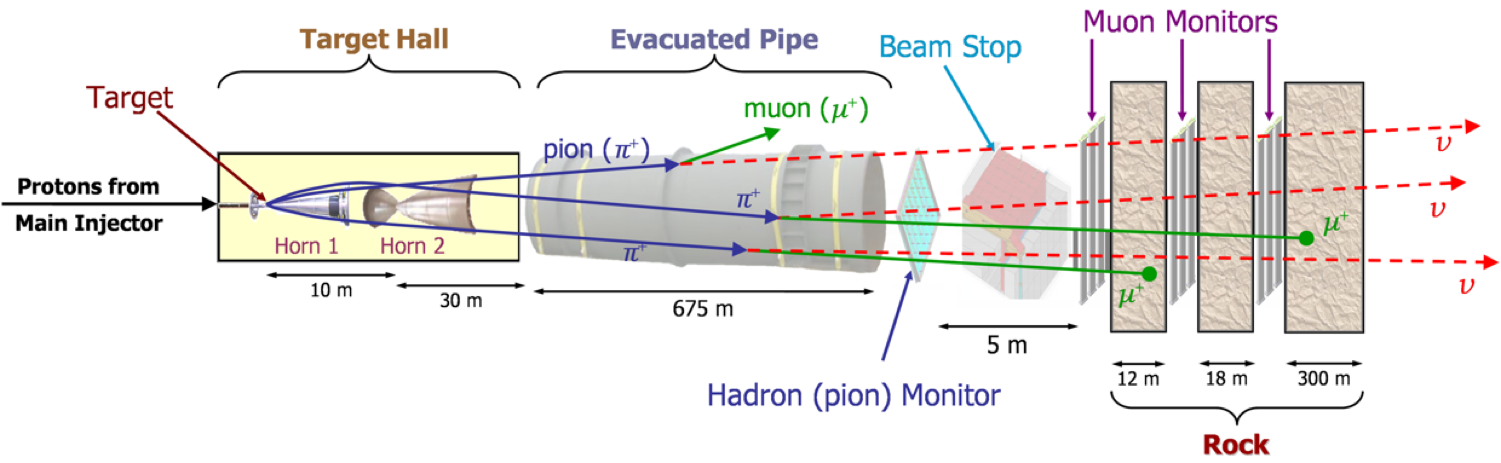
\includegraphics[width=\textwidth]{figures/beam.png}
\end{figure}
\begin{itemize}
  \item 120 GeV proton on carbon target, POT = Protons on Target
  \item Horn pulsed at -200 kA (or +200 kA to make anti-neutrino beam)
  \item Every 1.3 s we get 6 batches of protons from Booster on the target = 1 beam spill
  \item 10 $\mu$s of beam = 1 beam spill
  \item Every time we are going to get this 10 $\mu$s of beam the people at accelerator division sends us a signal letting us know.
\end{itemize}
\end{frame}

\begin{frame}{Near Detector Location}
\begin{figure}
\centering
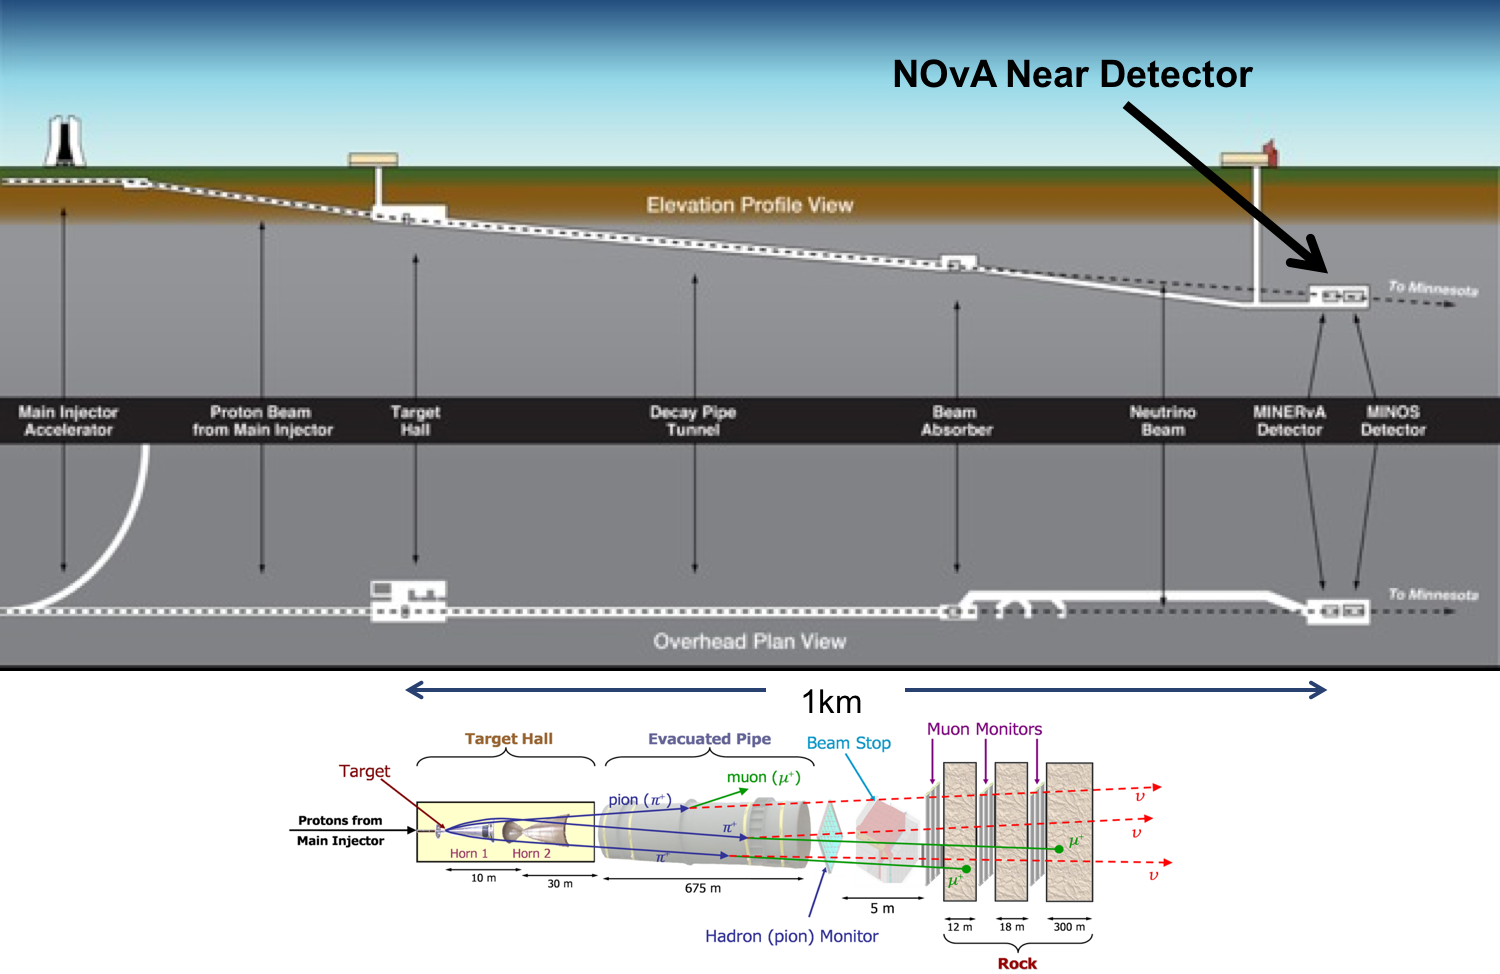
\includegraphics[width=\textwidth]{figures/nd_position.png}
\end{figure}
NO$\nu$A near detector is 1 km from the target 105 m underground.
\end{frame}

\begin{frame}{NO$\nu$A Off-axis Beam}
\begin{figure}
\centering
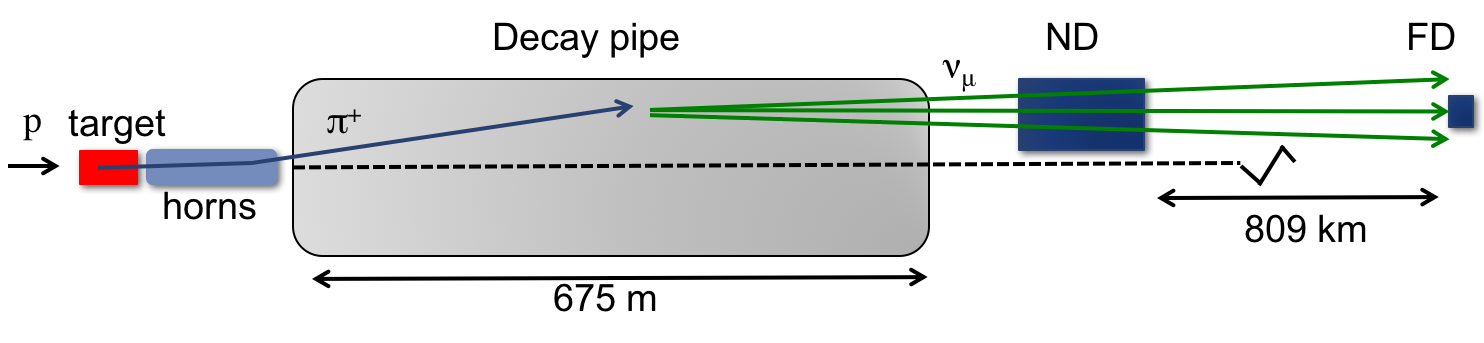
\includegraphics[width=\textwidth]{figures/nd_off_axis.png}
\end{figure}
\begin{figure}
\centering
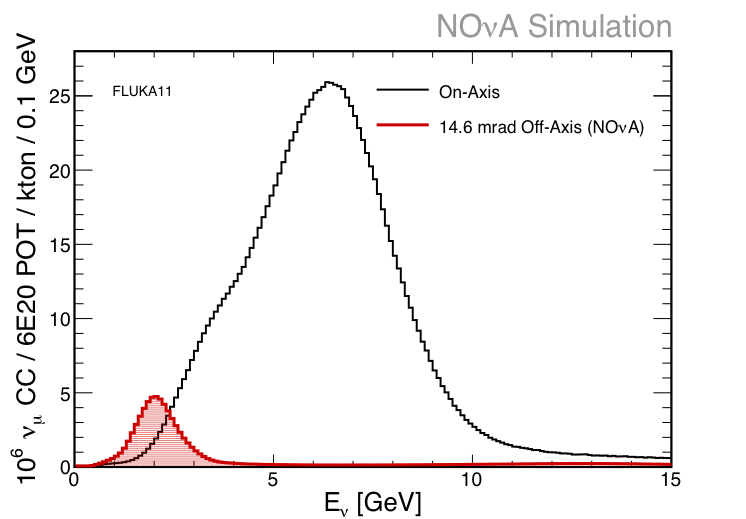
\includegraphics[width=.6\textwidth]{figures/nd_nu_spec.png}
\end{figure}
\end{frame}

\begin{frame}{Detector Dimensions}
\begin{figure}
  \centering
  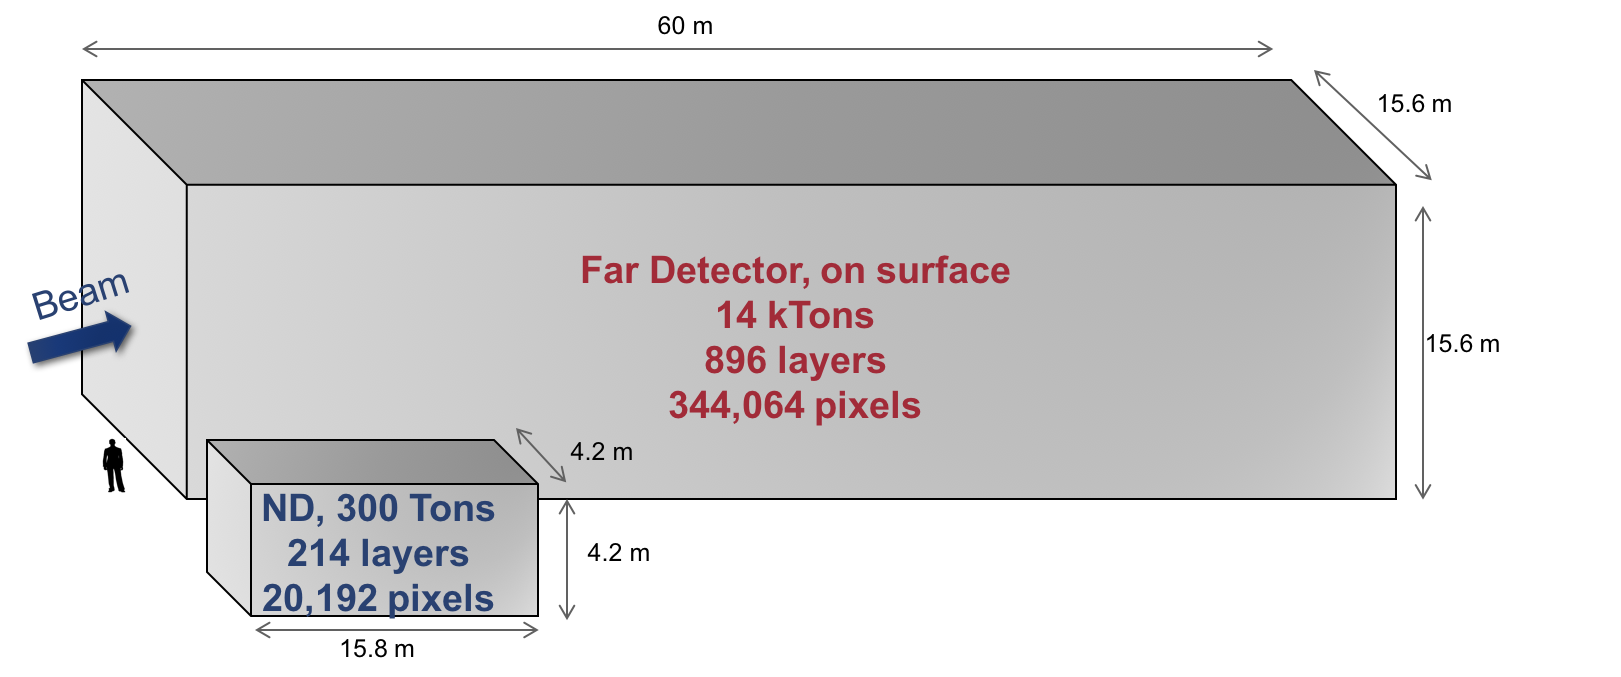
\includegraphics[width=\textwidth]{figures/detector_sizes.png}
\end{figure}
Two functionally identical 65\% active low-Z tracking calorimeters
\end{frame}

\begin{frame}{Detector Cells}
\begin{figure}
  \centering
  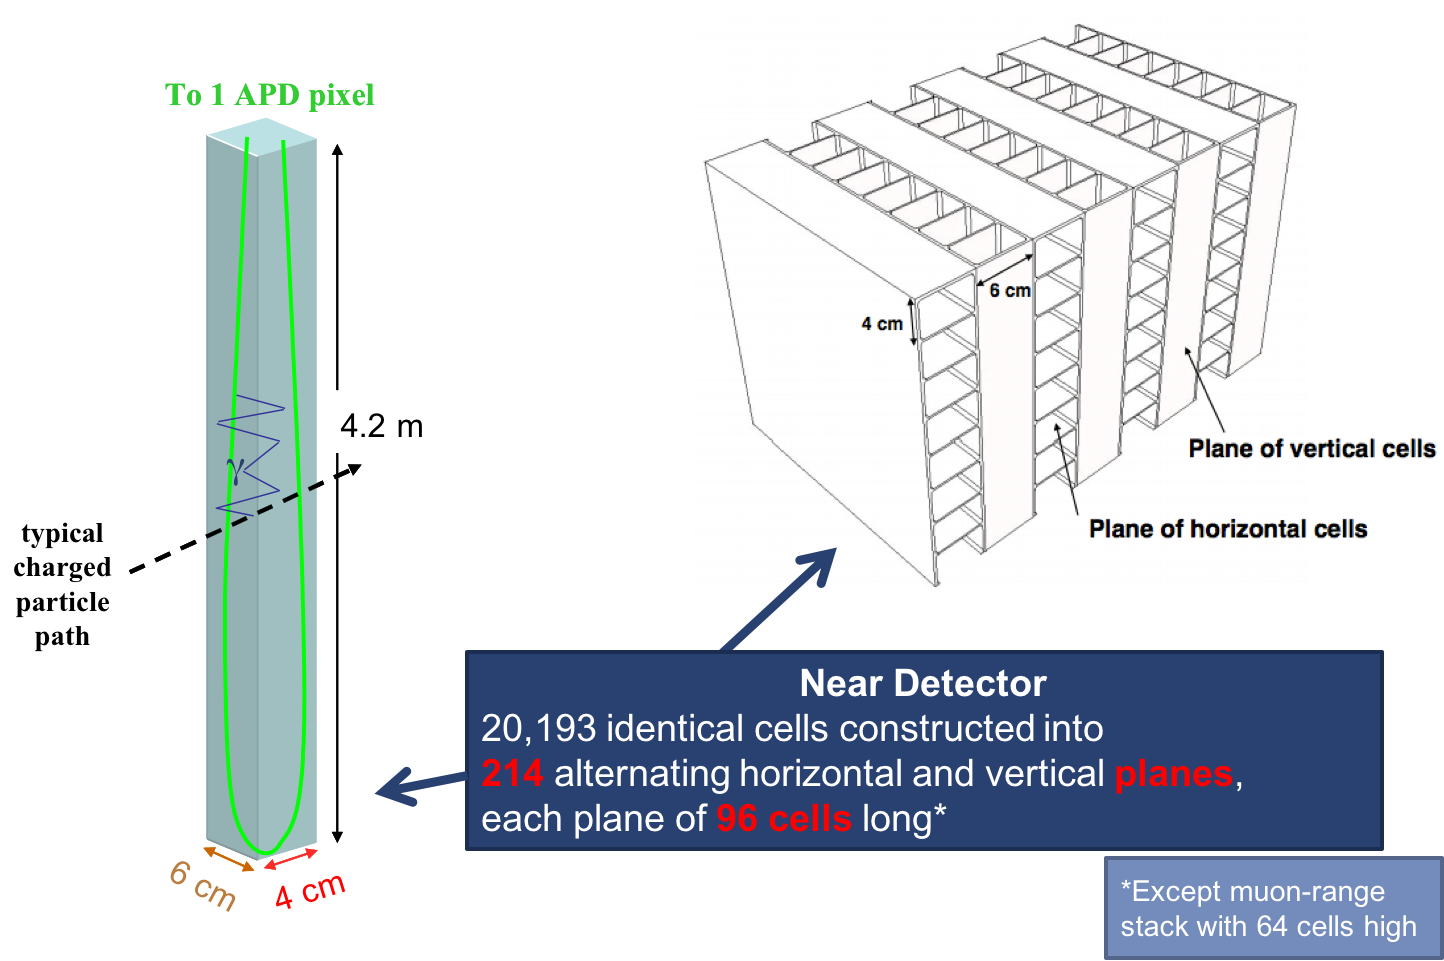
\includegraphics[width=\textwidth]{figures/nd_cells.png}
\end{figure}
\small
Cells constructed into horizontal and vertical planes for 3D reconstruction
\end{frame}

\begin{frame}{NO$\nu$A Scintillator}
\begin{itemize}
  \item material producing light when a charged particle travels through it
  \item by mass NO$\nu$A scintillator is mostly mineral oil solvent
  \item blended into the mineral oil are a primary scintillant to generate UV light and two wavelength shifters converting UV to blue light
  \item wavelength shifting fiber shifts blue to green light and guides the light to avalanche photodetectors
  \item light yield is modeled by the Birks-Chou model
  \begin{equation*}
    \frac{dL}{dx}=\frac{L_0 \frac{dE}{dx}}{1+k_B\frac{dE}{dx}+k_C\left(\frac{dE}{dx}\right)^2}
  \end{equation*}
\end{itemize}
\end{frame}

\begin{frame}{Event Schematic}
\begin{figure}
  \centering
  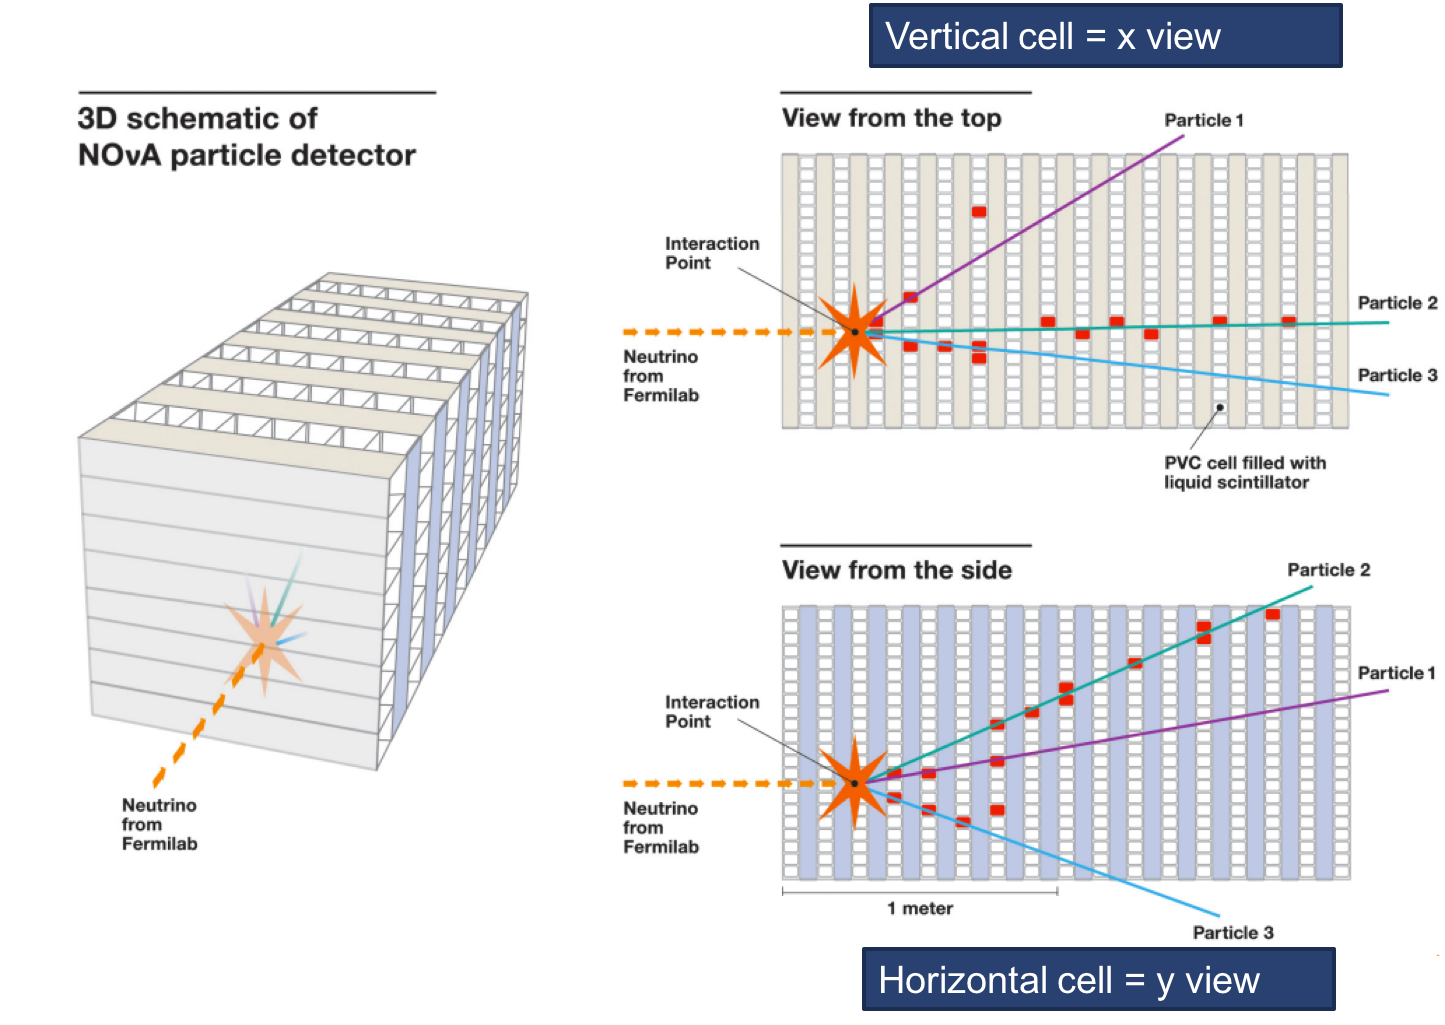
\includegraphics[width=\textwidth]{figures/schematic.png}
\end{figure}
\end{frame}

\begin{frame}{Neutrino Event Topology}
\begin{figure}
  \centering
  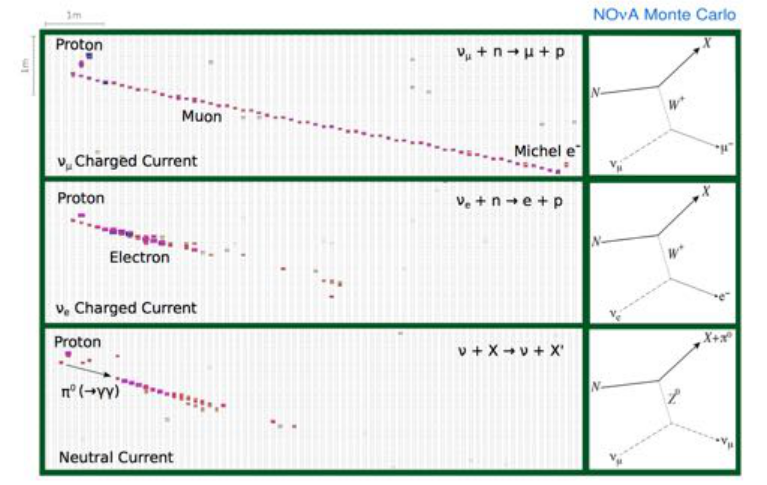
\includegraphics[width=\textwidth]{figures/topology.png}
\end{figure}
\begin{enumerate}
  \scriptsize
  \item the muon leaves a long minimum ionizing particle (MIP) track
  \item the electron ionizes in the first few planes before starting a shower
  \item the pion is a shower with a gap in the first few plane
\end{enumerate}
\end{frame}

\begin{frame}{$\nu_\mu$ Charged Current Signal Event Display}
\begin{figure}
\centering
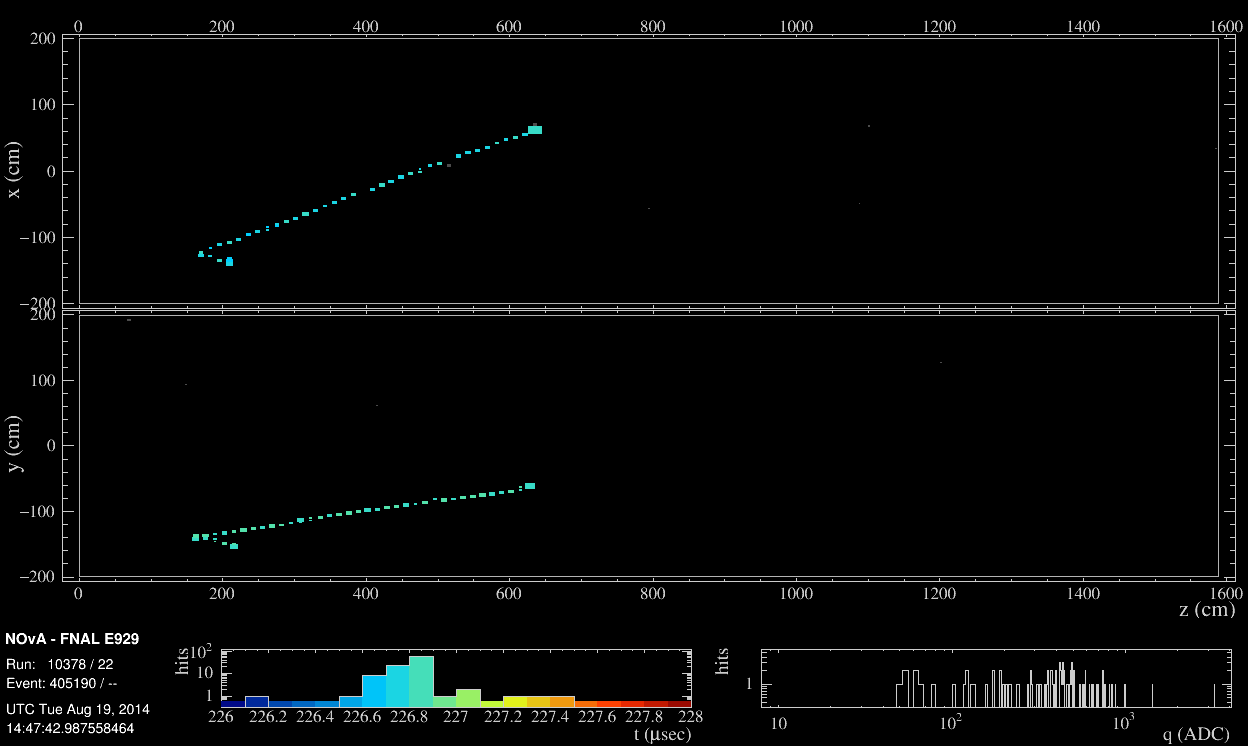
\includegraphics[width=\textwidth]{figures/numucc_signal.png}
\end{figure}
\end{frame}

\begin{frame}{$\bar{\nu}_\mu$ Charged Current Event Selection}
\begin{enumerate}
  \item quality cut:\\
  requires a track to be reconstructed, removes low cell hits events, and removes vertical events, etc.
  \item containment cut:\\
  requires the muon track to be contained in the detector
  \item particle identification (PID):\\
  Where all tricks are.
\end{enumerate}
\end{frame}

\begin{frame}{Reconstructed Muon Identification (ReMId)}
\begin{itemize}
  \item ReMId uses a k-Nearest Neighbors (kNN) algorithm to make its determination.
  \item input variables are
  \begin{itemize}
    \item log-likelihoods using the $\frac{dE}{dx}$ of the track
    \item log-likelihoods bases on the scattering observed in the track
    \item the track length
    \item the fraction of planes used to create the $\frac{dE}{dx}$ log-likelihood
  \end{itemize}
  \item The kNN returns a value between 0 and 1, 1 being muon-like and 0 being background-like.
  \item A cut value is optimized to minimize the statistical error on the parameter interested.
\end{itemize}
\end{frame}

\begin{frame}{ReMId Distributions for Different Modes}
\begin{figure}
  \centering
  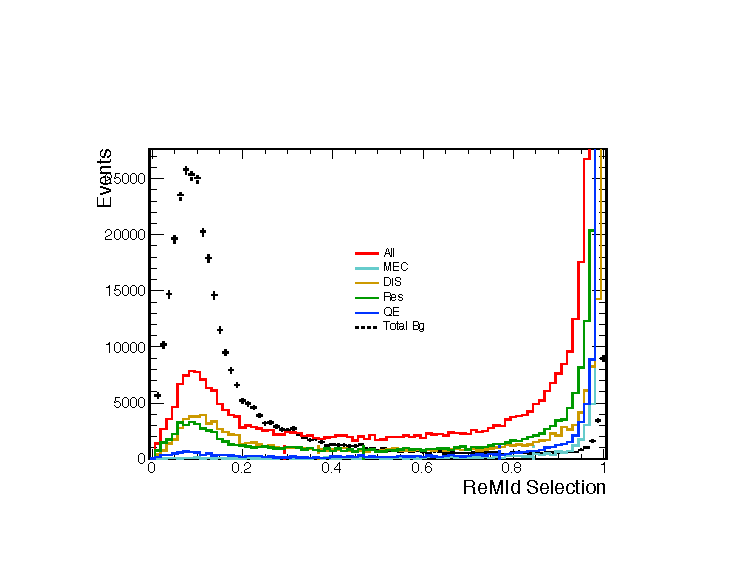
\includegraphics[width=\textwidth]{figures/remid.pdf}
\end{figure}
\end{frame}

\begin{frame}{Event Selection on Monte Carlo}
\begin{figure}
  \centering
  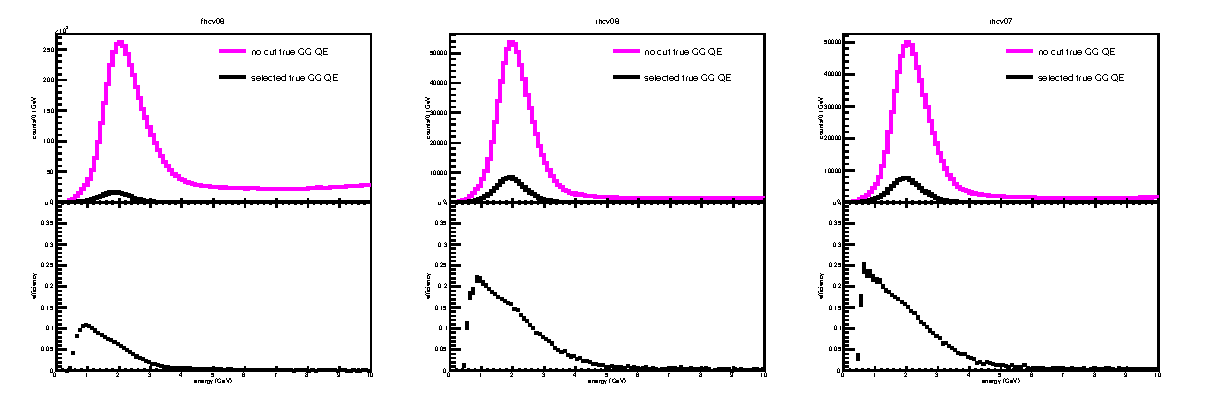
\includegraphics[width=\textwidth]{figures/eff.eps}
\end{figure}
Cut used: Quality + Containment + ReMId
\end{frame}

\begin{frame}{Items Contributing to the Uncertainties of Cross Section Measurement}
\begin{itemize}
  \item Geant4 nuclear model:\\ particles from CC interactions undergo rescattering in the nuclei
  \item Birks parameter tuning:\\ energy calibration
  \item energy scale:\\ how well the neutrino energy is reconstructed
  \item flux uncertainties
  \item rock events:\\ neutrino interactions outside of the detector entering the detector
  \item GENIE:\\ neutrino event generator involving model dependencies
\end{itemize}
\end{frame}

\begin{frame}[c]
\begin{center}
\Huge Thank you!
\end{center}
\end{frame}

\end{document}